% Options for packages loaded elsewhere
\PassOptionsToPackage{unicode}{hyperref}
\PassOptionsToPackage{hyphens}{url}
%
\documentclass[
]{article}
\usepackage{amsmath,amssymb}
\usepackage{iftex}
\ifPDFTeX
  \usepackage[T1]{fontenc}
  \usepackage[utf8]{inputenc}
  \usepackage{textcomp} % provide euro and other symbols
\else % if luatex or xetex
  \usepackage{unicode-math} % this also loads fontspec
  \defaultfontfeatures{Scale=MatchLowercase}
  \defaultfontfeatures[\rmfamily]{Ligatures=TeX,Scale=1}
\fi
\usepackage{lmodern}
\ifPDFTeX\else
  % xetex/luatex font selection
\fi
% Use upquote if available, for straight quotes in verbatim environments
\IfFileExists{upquote.sty}{\usepackage{upquote}}{}
\IfFileExists{microtype.sty}{% use microtype if available
  \usepackage[]{microtype}
  \UseMicrotypeSet[protrusion]{basicmath} % disable protrusion for tt fonts
}{}
\makeatletter
\@ifundefined{KOMAClassName}{% if non-KOMA class
  \IfFileExists{parskip.sty}{%
    \usepackage{parskip}
  }{% else
    \setlength{\parindent}{0pt}
    \setlength{\parskip}{6pt plus 2pt minus 1pt}}
}{% if KOMA class
  \KOMAoptions{parskip=half}}
\makeatother
\usepackage{xcolor}
\usepackage[margin=1in]{geometry}
\usepackage{color}
\usepackage{fancyvrb}
\newcommand{\VerbBar}{|}
\newcommand{\VERB}{\Verb[commandchars=\\\{\}]}
\DefineVerbatimEnvironment{Highlighting}{Verbatim}{commandchars=\\\{\}}
% Add ',fontsize=\small' for more characters per line
\usepackage{framed}
\definecolor{shadecolor}{RGB}{248,248,248}
\newenvironment{Shaded}{\begin{snugshade}}{\end{snugshade}}
\newcommand{\AlertTok}[1]{\textcolor[rgb]{0.94,0.16,0.16}{#1}}
\newcommand{\AnnotationTok}[1]{\textcolor[rgb]{0.56,0.35,0.01}{\textbf{\textit{#1}}}}
\newcommand{\AttributeTok}[1]{\textcolor[rgb]{0.13,0.29,0.53}{#1}}
\newcommand{\BaseNTok}[1]{\textcolor[rgb]{0.00,0.00,0.81}{#1}}
\newcommand{\BuiltInTok}[1]{#1}
\newcommand{\CharTok}[1]{\textcolor[rgb]{0.31,0.60,0.02}{#1}}
\newcommand{\CommentTok}[1]{\textcolor[rgb]{0.56,0.35,0.01}{\textit{#1}}}
\newcommand{\CommentVarTok}[1]{\textcolor[rgb]{0.56,0.35,0.01}{\textbf{\textit{#1}}}}
\newcommand{\ConstantTok}[1]{\textcolor[rgb]{0.56,0.35,0.01}{#1}}
\newcommand{\ControlFlowTok}[1]{\textcolor[rgb]{0.13,0.29,0.53}{\textbf{#1}}}
\newcommand{\DataTypeTok}[1]{\textcolor[rgb]{0.13,0.29,0.53}{#1}}
\newcommand{\DecValTok}[1]{\textcolor[rgb]{0.00,0.00,0.81}{#1}}
\newcommand{\DocumentationTok}[1]{\textcolor[rgb]{0.56,0.35,0.01}{\textbf{\textit{#1}}}}
\newcommand{\ErrorTok}[1]{\textcolor[rgb]{0.64,0.00,0.00}{\textbf{#1}}}
\newcommand{\ExtensionTok}[1]{#1}
\newcommand{\FloatTok}[1]{\textcolor[rgb]{0.00,0.00,0.81}{#1}}
\newcommand{\FunctionTok}[1]{\textcolor[rgb]{0.13,0.29,0.53}{\textbf{#1}}}
\newcommand{\ImportTok}[1]{#1}
\newcommand{\InformationTok}[1]{\textcolor[rgb]{0.56,0.35,0.01}{\textbf{\textit{#1}}}}
\newcommand{\KeywordTok}[1]{\textcolor[rgb]{0.13,0.29,0.53}{\textbf{#1}}}
\newcommand{\NormalTok}[1]{#1}
\newcommand{\OperatorTok}[1]{\textcolor[rgb]{0.81,0.36,0.00}{\textbf{#1}}}
\newcommand{\OtherTok}[1]{\textcolor[rgb]{0.56,0.35,0.01}{#1}}
\newcommand{\PreprocessorTok}[1]{\textcolor[rgb]{0.56,0.35,0.01}{\textit{#1}}}
\newcommand{\RegionMarkerTok}[1]{#1}
\newcommand{\SpecialCharTok}[1]{\textcolor[rgb]{0.81,0.36,0.00}{\textbf{#1}}}
\newcommand{\SpecialStringTok}[1]{\textcolor[rgb]{0.31,0.60,0.02}{#1}}
\newcommand{\StringTok}[1]{\textcolor[rgb]{0.31,0.60,0.02}{#1}}
\newcommand{\VariableTok}[1]{\textcolor[rgb]{0.00,0.00,0.00}{#1}}
\newcommand{\VerbatimStringTok}[1]{\textcolor[rgb]{0.31,0.60,0.02}{#1}}
\newcommand{\WarningTok}[1]{\textcolor[rgb]{0.56,0.35,0.01}{\textbf{\textit{#1}}}}
\usepackage{graphicx}
\makeatletter
\def\maxwidth{\ifdim\Gin@nat@width>\linewidth\linewidth\else\Gin@nat@width\fi}
\def\maxheight{\ifdim\Gin@nat@height>\textheight\textheight\else\Gin@nat@height\fi}
\makeatother
% Scale images if necessary, so that they will not overflow the page
% margins by default, and it is still possible to overwrite the defaults
% using explicit options in \includegraphics[width, height, ...]{}
\setkeys{Gin}{width=\maxwidth,height=\maxheight,keepaspectratio}
% Set default figure placement to htbp
\makeatletter
\def\fps@figure{htbp}
\makeatother
\setlength{\emergencystretch}{3em} % prevent overfull lines
\providecommand{\tightlist}{%
  \setlength{\itemsep}{0pt}\setlength{\parskip}{0pt}}
\setcounter{secnumdepth}{-\maxdimen} % remove section numbering
\usepackage{booktabs}
\usepackage{longtable}
\usepackage{array}
\usepackage{multirow}
\usepackage{wrapfig}
\usepackage{float}
\usepackage{colortbl}
\usepackage{pdflscape}
\usepackage{tabu}
\usepackage{threeparttable}
\usepackage{threeparttablex}
\usepackage[normalem]{ulem}
\usepackage{makecell}
\usepackage{xcolor}
\ifLuaTeX
  \usepackage{selnolig}  % disable illegal ligatures
\fi
\IfFileExists{bookmark.sty}{\usepackage{bookmark}}{\usepackage{hyperref}}
\IfFileExists{xurl.sty}{\usepackage{xurl}}{} % add URL line breaks if available
\urlstyle{same}
\hypersetup{
  pdftitle={Foundational concepts for simulation studies},
  pdfauthor={Ian Hussey},
  hidelinks,
  pdfcreator={LaTeX via pandoc}}

\title{Foundational concepts for simulation studies}
\usepackage{etoolbox}
\makeatletter
\providecommand{\subtitle}[1]{% add subtitle to \maketitle
  \apptocmd{\@title}{\par {\large #1 \par}}{}{}
}
\makeatother
\subtitle{Populations, samples, pseudo-random number generators,
for-loops, and parameter recovery}
\author{Ian Hussey}
\date{01 Mai, 2024}

\begin{document}
\maketitle

\begin{Shaded}
\begin{Highlighting}[]
\CommentTok{\# dependencies}
\FunctionTok{library}\NormalTok{(tidyverse)}
\FunctionTok{library}\NormalTok{(scales)}
\FunctionTok{library}\NormalTok{(knitr)}
\FunctionTok{library}\NormalTok{(kableExtra)}
\FunctionTok{library}\NormalTok{(janitor)}
\CommentTok{\# install.packages("devtools")}
\CommentTok{\# library(devtools)}
\CommentTok{\# devtools::install\_github("ianhussey/simulateR")}
\FunctionTok{library}\NormalTok{(simulateR) }\CommentTok{\# available from github {-} uncomment the above lines to install}

\CommentTok{\# set seed}
\FunctionTok{set.seed}\NormalTok{(}\DecValTok{42}\NormalTok{)}
\end{Highlighting}
\end{Shaded}

\hypertarget{why-do-inferential-statistics}{%
\section{Why do inferential
statistics?}\label{why-do-inferential-statistics}}

Do these two groups differ from one another? Does the intervention group
have a lower average depression score than the control group?

These plots contain data that is simulated but realistic for a
hypothetical RCT comparing a psychotherapeutic intervention versus
waiting list control. The (hypothetical) outcome variable is a popular
measure of depression, the Beck Depression Inventory II.

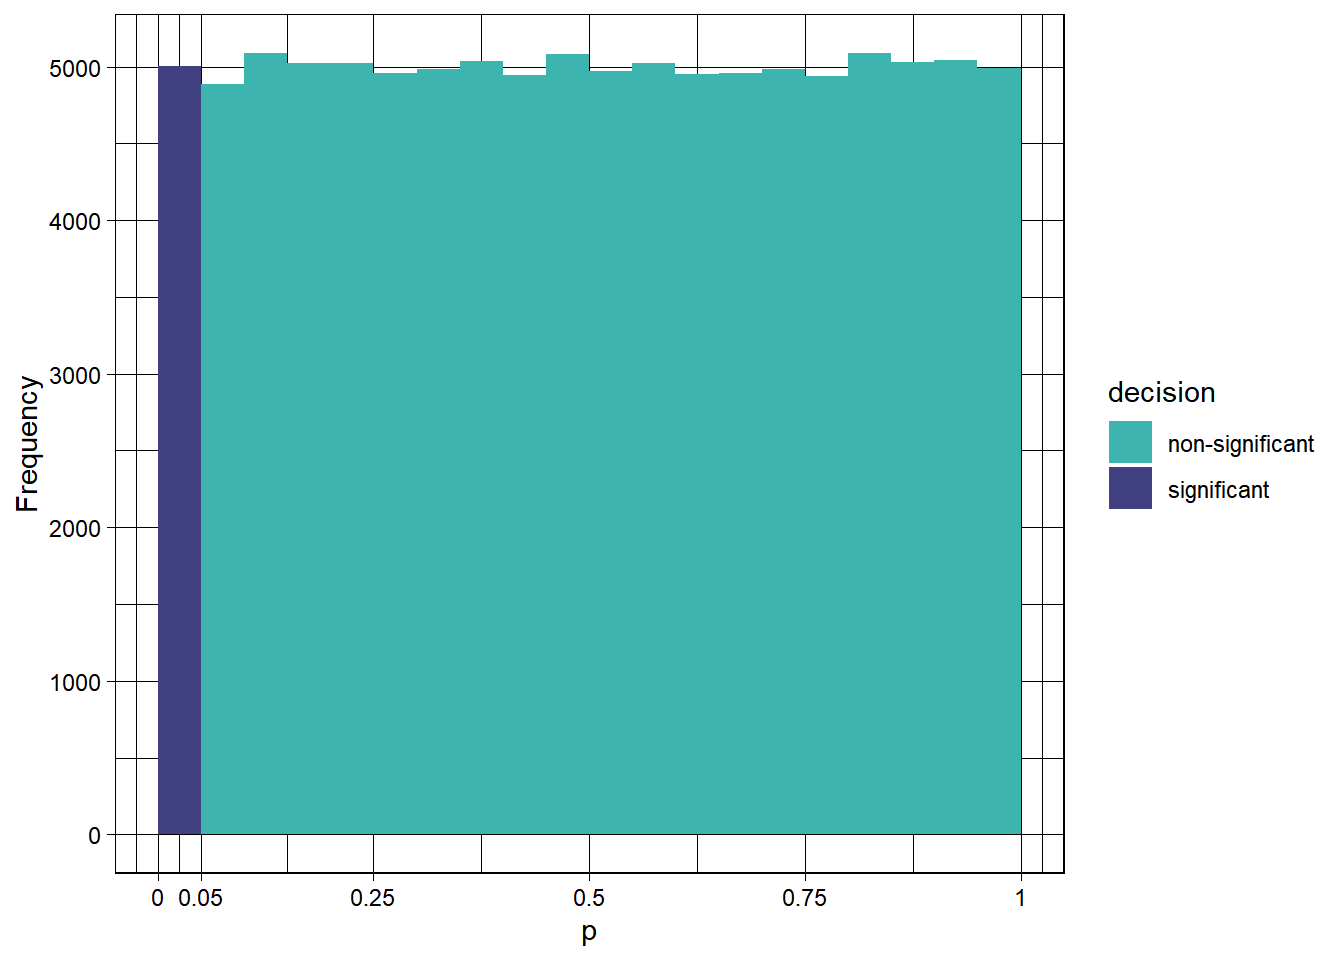
\includegraphics{1_foundational_concepts__lesson_files/figure-latex/unnamed-chunk-1-1.pdf}

Statistical inference is about making inferences about populations from
limited samples drawn from those populations.

Generally speaking, psychology studies are less interested in the
specific participants that we study, and more interested in making
generalisations about the populations they are drawn from. E.g., would
people in general, other than these participants we studied here,
benefit from this therapy?

The previous plots sampled 40 participants per condition from a true
population. Imagine we were able to see data from the whole population -
which we never can in real life.

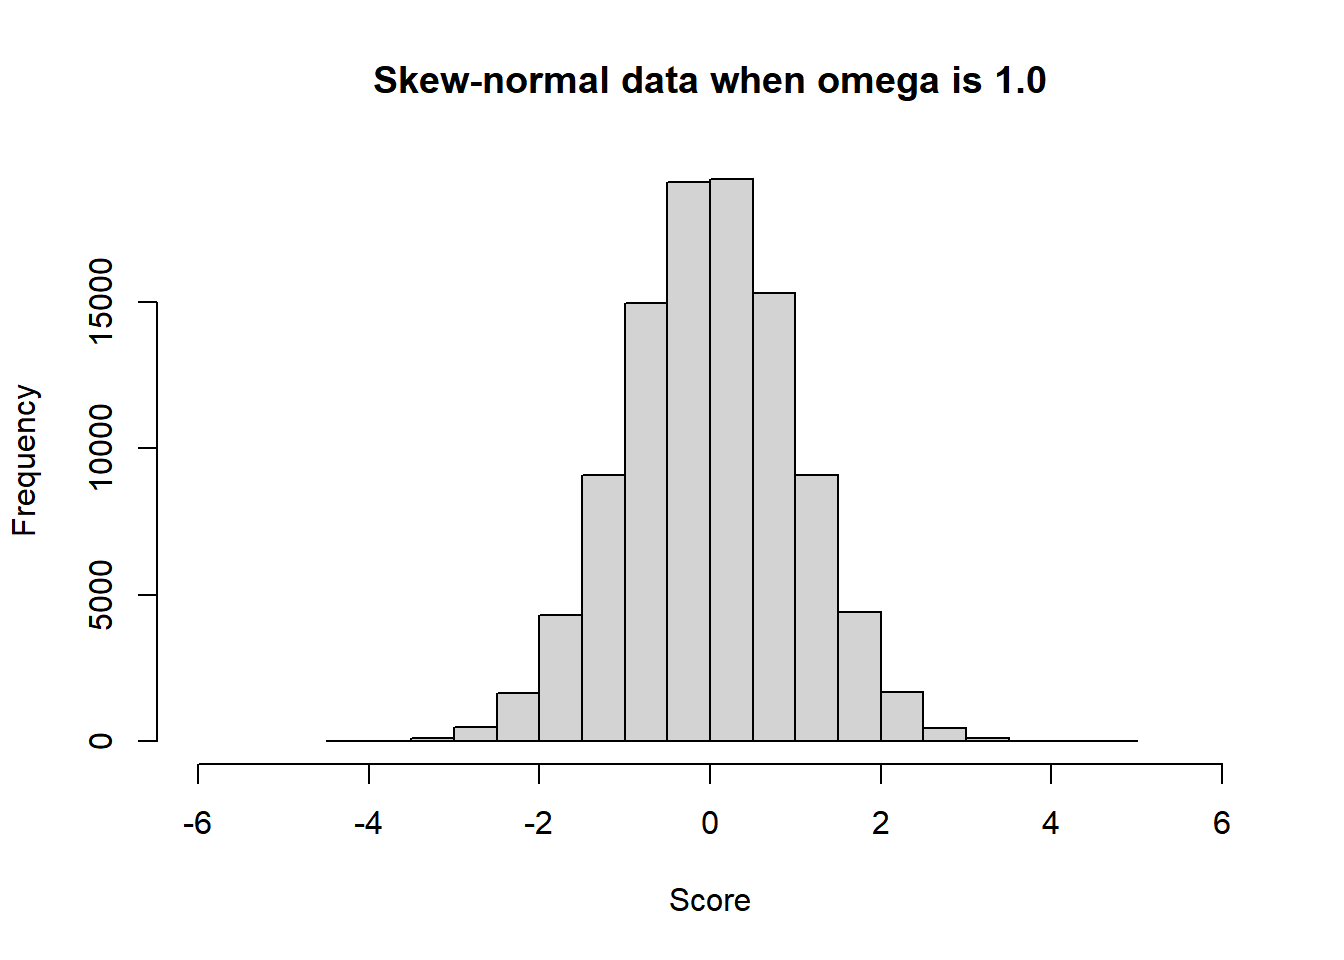
\includegraphics{1_foundational_concepts__lesson_files/figure-latex/unnamed-chunk-2-1.pdf}

It's easier to see from this plot that the therapy does indeed work. The
values are also realistic: the means, SDs, and effect sizes are
reasonable for BDI-II scores for an effective therapy. Unfortunately, we
almost never have access to the full population we are interested in
knowing about. Inferential statistics allow us to use data from smaller
samples to make inferences about the larger populations they are drawn
from.

\hypertarget{why-do-stimulation-studies}{%
\section{Why do stimulation studies?}\label{why-do-stimulation-studies}}

When you apply an inferential test to real-world data, you are never
sure whether the result of your test is truly correct or not, you can
only make probability statements about being right (e.g., the long-run
false-positive rate, controlled using a test's alpha value). This makes
it hard to know if statistical tests are working correctly as planned,
because you never have access to ground-truth.

Simulation studies are very useful because they allow you to construct
this ground truth and then apply tests to it. If you're interested in
knowing whether your statistical test is good at detecting population
effects of a given size in small sample sizes, you can create an
arbitrary number of samples drawn from this precise population.

To take a concrete example: we are often taught that ``violating
statistical assumptions is bad'' in some way. But how severe is the
violation, and how negative a consequence does this have? In what
contexts, and why? Simulation lets you answer questions like these. In
doing so, it can change our understanding of statistical analyses from a
set of rules we have learned to a deeper and principled understanding of
why we are choosing to analyse data in a given way.

\hypertarget{pseudo-random-number-generators}{%
\section{Pseudo-random number
generators}\label{pseudo-random-number-generators}}

Randomness is impossible to achieve. All ``random'' number generators
are actually pseudo-random number generators (PRNGs). Computer
scientists and mathematicians spend lots of time trying to increase the
randomness of our random number generators, because any degree of
predictability adds bias to any models built on them. Pseudo-random
numbers are at the core of simulation studies, as they allow us to
(pseudo) randomly sample simulated data from known population
distributions.

\hypertarget{sampling-from-uniform-distributions}{%
\subsection{Sampling from uniform
distributions}\label{sampling-from-uniform-distributions}}

A uniform distributions is when every value is as likely as every other
value, and are selected from a given range. E.g., ``pick a number
between 1 and 10'' where the picker is just as likely to say ``1'' as
any other number in that range.

\texttt{runif()} is a random generation function (the ``r'' part) for a
uniform distribution (the ``unif'' part). Not `run if', which confuses
some people.

So, this code, which generates a random number between 1 and 10, will
generate 3s just as often as it generates 7s. You can re run this code
yourself many times to see it generate different numbers between 1 and
10.

\begin{Shaded}
\begin{Highlighting}[]
\FunctionTok{runif}\NormalTok{(}\AttributeTok{n =} \DecValTok{1}\NormalTok{, }
      \AttributeTok{min =} \DecValTok{1}\NormalTok{,}
      \AttributeTok{max =} \DecValTok{10}\NormalTok{) }\SpecialCharTok{|\textgreater{}}
  \FunctionTok{round\_half\_up}\NormalTok{(}\DecValTok{0}\NormalTok{)}
\end{Highlighting}
\end{Shaded}

\begin{verbatim}
## [1] 7
\end{verbatim}

\hypertarget{random-number-generators-are-not-truly-random}{%
\section{Random number generators are not truly
random}\label{random-number-generators-are-not-truly-random}}

You don't need to understand how PRNGs work, but you do need to know
that the these ``random'' numbers can be predictably reproduced. The
`seed' value from which a PRNG starts can be set to control which random
numbers are generated.

\begin{Shaded}
\begin{Highlighting}[]
\FunctionTok{set.seed}\NormalTok{(}\DecValTok{43}\NormalTok{) }\CommentTok{\# set the starting seed value for generating the random numbers}

\FunctionTok{runif}\NormalTok{(}\AttributeTok{n =} \DecValTok{1}\NormalTok{, }
      \AttributeTok{min =} \DecValTok{1}\NormalTok{,}
      \AttributeTok{max =} \DecValTok{10}\NormalTok{) }\SpecialCharTok{|\textgreater{}}
  \FunctionTok{round\_half\_up}\NormalTok{(}\DecValTok{0}\NormalTok{)}
\end{Highlighting}
\end{Shaded}

\begin{verbatim}
## [1] 5
\end{verbatim}

\begin{Shaded}
\begin{Highlighting}[]
\FunctionTok{set.seed}\NormalTok{(}\DecValTok{43}\NormalTok{) }\CommentTok{\# set it again to the same value starting seed value for generating the random numbers}

\FunctionTok{runif}\NormalTok{(}\AttributeTok{n =} \DecValTok{1}\NormalTok{, }
      \AttributeTok{min =} \DecValTok{1}\NormalTok{,}
      \AttributeTok{max =} \DecValTok{10}\NormalTok{) }\SpecialCharTok{|\textgreater{}}
  \FunctionTok{round\_half\_up}\NormalTok{(}\DecValTok{0}\NormalTok{)}
\end{Highlighting}
\end{Shaded}

\begin{verbatim}
## [1] 5
\end{verbatim}

Note that if you run the function a second time without resetting to a
known seed, the second value will be different to the first one.

\begin{Shaded}
\begin{Highlighting}[]
\FunctionTok{set.seed}\NormalTok{(}\DecValTok{43}\NormalTok{) }\CommentTok{\# set the starting seed value for generating the random numbers}

\FunctionTok{runif}\NormalTok{(}\AttributeTok{n =} \DecValTok{1}\NormalTok{, }
      \AttributeTok{min =} \DecValTok{1}\NormalTok{,}
      \AttributeTok{max =} \DecValTok{10}\NormalTok{) }\SpecialCharTok{|\textgreater{}}
  \FunctionTok{round\_half\_up}\NormalTok{(}\DecValTok{0}\NormalTok{)}
\end{Highlighting}
\end{Shaded}

\begin{verbatim}
## [1] 5
\end{verbatim}

\begin{Shaded}
\begin{Highlighting}[]
\FunctionTok{runif}\NormalTok{(}\AttributeTok{n =} \DecValTok{1}\NormalTok{, }
      \AttributeTok{min =} \DecValTok{1}\NormalTok{,}
      \AttributeTok{max =} \DecValTok{10}\NormalTok{) }\SpecialCharTok{|\textgreater{}}
  \FunctionTok{round\_half\_up}\NormalTok{(}\DecValTok{0}\NormalTok{)}
\end{Highlighting}
\end{Shaded}

\begin{verbatim}
## [1] 9
\end{verbatim}

This is because the Nth value of any sequence from a given seed is
knowable, whether its run once or in multiple runs.

\begin{Shaded}
\begin{Highlighting}[]
\FunctionTok{set.seed}\NormalTok{(}\DecValTok{43}\NormalTok{) }\CommentTok{\# set the starting seed value for generating the random numbers}

\CommentTok{\# generate both of the above numbers in one function call}
\FunctionTok{runif}\NormalTok{(}\AttributeTok{n =} \DecValTok{2}\NormalTok{, }\CommentTok{\# generate two numbers rather than one}
      \AttributeTok{min =} \DecValTok{1}\NormalTok{,}
      \AttributeTok{max =} \DecValTok{10}\NormalTok{) }\SpecialCharTok{|\textgreater{}}
  \FunctionTok{round\_half\_up}\NormalTok{(}\DecValTok{0}\NormalTok{)}
\end{Highlighting}
\end{Shaded}

\begin{verbatim}
## [1] 5 9
\end{verbatim}

\hypertarget{sampling-from-normal-distributions}{%
\subsection{Sampling from normal
distributions}\label{sampling-from-normal-distributions}}

\texttt{rnorm()} is a random generation function (the ``r'' part) for
normal distributions (the ``norm'' part).

Note that normal distributions are sometimes referred to as Gaussian
distributions. This can be useful as it can rid us of the impression
that Gaussian distributions are typical/standard/default, or that other
distributions are abnormal in some way. However, ``normal'' is more
common so we'll use it.

\texttt{rnorm()} is like magic, because it allows you to create data
that follows the assumptions of our most common statistical analyses.
The difference between simulated data, e.g., from \texttt{rnorm()}, and
real data from participants, is that we can know what the real
population value - the data generating signals - are in simulated data.
Whereas with real participant data we don't ever know this for sure. We
use real data to make inferences - best guesses - about (unobserved,
unknowable) true populations.

The below code generates data from a normal distribution, where the
population mean (usually notated as \[\mu\] ) is 7.52 and the population
standard deviation (usually noted as \(\sigma\)) is 3.18. Let's sample
100 simulated ``participants''.

\begin{Shaded}
\begin{Highlighting}[]
\CommentTok{\#$$\textbackslash{}mu$$ {-}\textgreater{} mu symbol $$\textbackslash{}sigma$$ {-}\textgreater{} sigma symbol}

\FunctionTok{rnorm}\NormalTok{(}\AttributeTok{n =} \DecValTok{100}\NormalTok{, }
      \AttributeTok{mean =} \FloatTok{7.52}\NormalTok{, }
      \AttributeTok{sd =} \FloatTok{3.18}\NormalTok{)}
\end{Highlighting}
\end{Shaded}

\begin{verbatim}
##   [1]  2.5127580  5.9746233  8.9992922  4.6449681  6.6377637  8.7488614
##   [7]  7.3279149  5.3379484  1.4584850 13.2559560  4.4453442  6.3970839
##  [13] 11.0400612  9.3209115 14.0845018 12.1923034  2.2682295  8.1643840
##  [19]  5.2272841  7.0142457  9.8549099  6.3646957  7.4879010  9.3732909
##  [25]  6.5873431  3.0858640  7.2494402  5.3318568  5.0506602 13.0666590
##  [31]  8.9718465  7.1441995 12.8478098  3.8345012  7.3908623 10.9827326
##  [37] 12.3285839 10.3364826  8.5203292 13.5059072  6.2019522  4.6132806
##  [43]  9.2641947  4.9493314  9.2013831  8.7541560  6.7459866  5.9333882
##  [49]  7.6283154  8.4542556  8.7938039  6.9650353  8.2835166  3.5734530
##  [55]  0.8822097  5.9012722  7.5620074  4.3220909 10.8450172  7.1096607
##  [61]  7.6058013  7.3282377  9.2515998 10.0033800  3.7063326  3.3847643
##  [67]  8.1233128  4.1991932  9.4244811 10.4642459  9.4238010  8.3643321
##  [73]  6.6275344  8.1354815 12.9231734  7.9451509  3.5126656  7.9916667
##  [79]  9.8873840  7.2659647  5.4109653  3.9660905  1.1826540  9.9667953
##  [85] 11.0521923 12.6627685  9.3208589  2.3869794  5.2934703 11.4747428
##  [91] 13.0419833  7.9750700  9.2221276  5.5052833  6.3293344  6.5556286
##  [97] 14.0296200  7.2754612 15.8419109  4.8086489
\end{verbatim}

\hypertarget{parameter-recovery}{%
\subsection{Parameter recovery}\label{parameter-recovery}}

But \ldots{} how do we know that \texttt{rnorm()} actually does what it
claims to? How do we know it generates data with the parameters we tell
it to, and from a normal distribution?

-\textgreater{} By checking!

Generate a \emph{very large} sample of participants from a known
population (i.e., specified by the arguments given to \texttt{rnorm()}),
then quantify if those parameters are what is found in the simulated
data.

This ability to compare a known ground truth with what is observed in
the simulated data is called \textbf{parameter recovery}.

For example, the following code defines a population mean (\(\mu\) =
7.52) and population SD (\(\sigma\) = 3.18), simulates 1 million
participants from this population, and the calculates the mean and SD in
the sample. In such a large sample, the sample summary statistics should
be almost equal to the population that it was drawn from \emph{if the
\texttt{rnorm()} function does as it claims to}. This is an extremely
simple form of simulation study where, rather than take R for its word
that \texttt{rnorm()} samples correctly, we test it for ourselves.

\begin{Shaded}
\begin{Highlighting}[]
\NormalTok{simulated\_scores }\OtherTok{\textless{}{-}} \FunctionTok{rnorm}\NormalTok{(}\AttributeTok{n =} \DecValTok{1000000}\NormalTok{, }\CommentTok{\# note that we need lots and lots of data to get a precise estimate }
                          \AttributeTok{mean =} \FloatTok{7.52}\NormalTok{, }
                          \AttributeTok{sd =} \FloatTok{3.18}\NormalTok{)}

\FunctionTok{mean}\NormalTok{(simulated\_scores) }\SpecialCharTok{|\textgreater{}} \FunctionTok{round\_half\_up}\NormalTok{(}\DecValTok{2}\NormalTok{)}
\end{Highlighting}
\end{Shaded}

\begin{verbatim}
## [1] 7.52
\end{verbatim}

\begin{Shaded}
\begin{Highlighting}[]
\FunctionTok{sd}\NormalTok{(simulated\_scores) }\SpecialCharTok{|\textgreater{}} \FunctionTok{round\_half\_up}\NormalTok{(}\DecValTok{2}\NormalTok{)}
\end{Highlighting}
\end{Shaded}

\begin{verbatim}
## [1] 3.18
\end{verbatim}

Having access to the ground truth (the true population effect), i.e.,
being able to control the data generation process and then check that
your tests recover these properties, is at the heart of simulation
studies. It is the special magic that allows you to be confident that
you understand what a given analysis can and can't do, that you're using
it correctly.

\hypertarget{plotting-the-normal-distribution}{%
\subsection{Plotting the normal
distribution}\label{plotting-the-normal-distribution}}

Summary statistics like \texttt{mean()} and \texttt{sd()} allow us to
check that we have recovered those population parameters. But
\texttt{rnorm()} also claims to sample data from a specific
distribution: the normal distribution. Rather than take
\texttt{rnorm()}'s word for this, we still need to examine the
distribution of the data it generates to check that it is indeed
normally distributed. It is also just generally useful to be able to
plot distribution of simulated data. So, I have created some helper
functions that allow you to make these plots in just a line or two of
code.

\hypertarget{basic-ggplot}{%
\subsection{Basic ggplot}\label{basic-ggplot}}

Ok, but a little ugly. Making it prettier would mean lots more lines of
code.

\begin{Shaded}
\begin{Highlighting}[]
\NormalTok{simulated\_scores }\OtherTok{\textless{}{-}} 
  \FunctionTok{rnorm}\NormalTok{(}\AttributeTok{n =} \DecValTok{1000000}\NormalTok{, }\CommentTok{\# sample n}
        \AttributeTok{mean =} \DecValTok{0}\NormalTok{, }\CommentTok{\# population mean (μ or mu)}
        \AttributeTok{sd =} \DecValTok{1}\NormalTok{) }\CommentTok{\# population sd (σ or sigma)}

\NormalTok{dat }\OtherTok{\textless{}{-}} \FunctionTok{data.frame}\NormalTok{(}\AttributeTok{simulated\_scores =}\NormalTok{ simulated\_scores)}

\FunctionTok{ggplot}\NormalTok{(dat, }\FunctionTok{aes}\NormalTok{(}\AttributeTok{x =}\NormalTok{ simulated\_scores)) }\SpecialCharTok{+}
  \FunctionTok{geom\_histogram}\NormalTok{()}
\end{Highlighting}
\end{Shaded}

\includegraphics{1_foundational_concepts__lesson_files/figure-latex/unnamed-chunk-9-1.pdf}

\hypertarget{simulaterrnorm_histogram}{%
\subsection{simulateR::rnorm\_histogram()}\label{simulaterrnorm_histogram}}

The simulateR R package is in very early development. Its
\texttt{rnorm\_histogram()} function does both data generation and
plotting for you. It plots not only the sample summary statistics, but
also the parameters used to generate the data.

\begin{Shaded}
\begin{Highlighting}[]
\FunctionTok{rnorm\_histogram}\NormalTok{(}\AttributeTok{n =} \DecValTok{1000000}\NormalTok{, }
                \AttributeTok{mean =} \DecValTok{0}\NormalTok{, }
                \AttributeTok{sd =} \DecValTok{1}\NormalTok{)}
\end{Highlighting}
\end{Shaded}

\includegraphics{1_foundational_concepts__lesson_files/figure-latex/unnamed-chunk-10-1.pdf}

\hypertarget{understanding-mu-sigma-and-n}{%
\section{\texorpdfstring{Understanding \(\mu\), \(\sigma\), and
n}{Understanding \textbackslash mu, \textbackslash sigma, and n}}\label{understanding-mu-sigma-and-n}}

In order to really understand \texttt{rnorm()}'s parameters (\(\mu\),
\(\sigma\), and n) it useful to vary them.

\hypertarget{varying-the-population-mean-mu}{%
\subsection{\texorpdfstring{Varying the population mean
(\(\mu\))}{Varying the population mean (\textbackslash mu)}}\label{varying-the-population-mean-mu}}

As if wasn't already complicated enough, note that population mean
\(\mu\)) is also sometimes referred to as ``location''.

\begin{Shaded}
\begin{Highlighting}[]
\FunctionTok{rnorm\_histogram}\NormalTok{(}\AttributeTok{n =} \DecValTok{1000000}\NormalTok{, }
                \AttributeTok{mean =} \DecValTok{0}\NormalTok{, }
                \AttributeTok{sd =} \DecValTok{1}\NormalTok{) }
\end{Highlighting}
\end{Shaded}

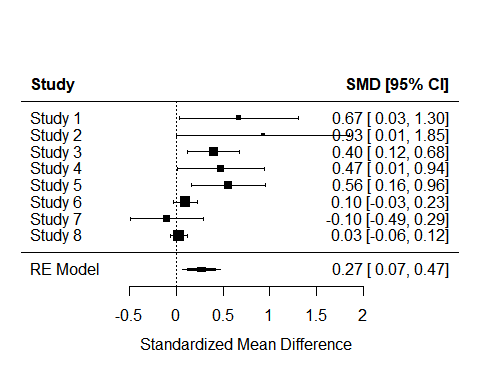
\includegraphics{1_foundational_concepts__lesson_files/figure-latex/unnamed-chunk-11-1.pdf}

\begin{Shaded}
\begin{Highlighting}[]
\FunctionTok{rnorm\_histogram}\NormalTok{(}\AttributeTok{n =} \DecValTok{1000000}\NormalTok{, }
                \AttributeTok{mean =} \SpecialCharTok{{-}}\DecValTok{2}\NormalTok{, }
                \AttributeTok{sd =} \DecValTok{1}\NormalTok{, }
                \AttributeTok{fill =} \StringTok{"darkcyan"}\NormalTok{) }
\end{Highlighting}
\end{Shaded}

\includegraphics{1_foundational_concepts__lesson_files/figure-latex/unnamed-chunk-11-2.pdf}

\hypertarget{varying-the-population-sd-sigma}{%
\subsection{\texorpdfstring{Varying the population SD
(\(\sigma\))}{Varying the population SD (\textbackslash sigma)}}\label{varying-the-population-sd-sigma}}

As if wasn't already complicated enough, note that population SD
\(\sigma\)) is closely related to the concept of variance, and both are
ways of talking about dispersion (i.e., spread) of scores around means.

\begin{Shaded}
\begin{Highlighting}[]
\FunctionTok{rnorm\_histogram}\NormalTok{(}\AttributeTok{n =} \DecValTok{1000000}\NormalTok{, }
                \AttributeTok{mean =} \DecValTok{0}\NormalTok{, }
                \AttributeTok{sd =} \DecValTok{1}\NormalTok{) }
\end{Highlighting}
\end{Shaded}

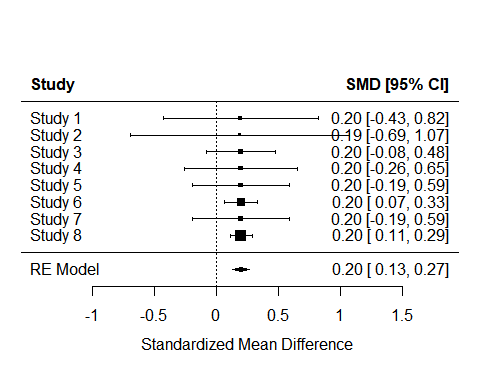
\includegraphics{1_foundational_concepts__lesson_files/figure-latex/unnamed-chunk-12-1.pdf}

\begin{Shaded}
\begin{Highlighting}[]
\FunctionTok{rnorm\_histogram}\NormalTok{(}\AttributeTok{n =} \DecValTok{1000000}\NormalTok{, }
                \AttributeTok{mean =} \DecValTok{0}\NormalTok{, }
                \AttributeTok{sd =} \DecValTok{2}\NormalTok{, }
                \AttributeTok{fill =} \StringTok{"darkcyan"}\NormalTok{) }
\end{Highlighting}
\end{Shaded}

\includegraphics{1_foundational_concepts__lesson_files/figure-latex/unnamed-chunk-12-2.pdf}

\hypertarget{varying-both-the-population-mean-mu-and-sd-sigma}{%
\subsection{\texorpdfstring{Varying both the population mean (\(\mu\))
and SD
(\(\sigma\))}{Varying both the population mean (\textbackslash mu) and SD (\textbackslash sigma)}}\label{varying-both-the-population-mean-mu-and-sd-sigma}}

\begin{Shaded}
\begin{Highlighting}[]
\FunctionTok{rnorm\_histogram}\NormalTok{(}\AttributeTok{n =} \DecValTok{1000000}\NormalTok{, }
                \AttributeTok{mean =} \DecValTok{0}\NormalTok{, }
                \AttributeTok{sd =} \DecValTok{1}\NormalTok{) }
\end{Highlighting}
\end{Shaded}

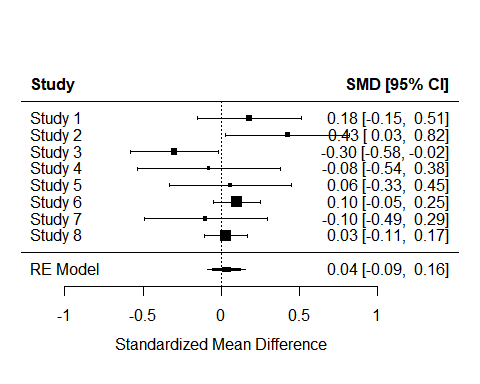
\includegraphics{1_foundational_concepts__lesson_files/figure-latex/unnamed-chunk-13-1.pdf}

\begin{Shaded}
\begin{Highlighting}[]
\FunctionTok{rnorm\_histogram}\NormalTok{(}\AttributeTok{n =} \DecValTok{1000000}\NormalTok{, }
                \AttributeTok{mean =} \SpecialCharTok{{-}}\DecValTok{2}\NormalTok{, }
                \AttributeTok{sd =} \DecValTok{2}\NormalTok{, }
                \AttributeTok{fill =} \StringTok{"darkcyan"}\NormalTok{) }
\end{Highlighting}
\end{Shaded}

\includegraphics{1_foundational_concepts__lesson_files/figure-latex/unnamed-chunk-13-2.pdf}

\hypertarget{varying-the-sample-n}{%
\subsection{Varying the sample N}\label{varying-the-sample-n}}

Aside from location and dispersion, we can also change the number of
simulated participants we sample from the population.

If we radically lower the sample sizes, from one million to one thousand
to one hundred, this will change how rough/granular/noisy the sampled
data looks, and how much the sample summary statistics (M and SD) differ
from the population parameters (\(\mu\) and \(\sigma\)).

\begin{Shaded}
\begin{Highlighting}[]
\FunctionTok{rnorm\_histogram}\NormalTok{(}\AttributeTok{n =} \DecValTok{1000000}\NormalTok{, }
                \AttributeTok{mean =} \DecValTok{0}\NormalTok{, }
                \AttributeTok{sd =} \DecValTok{1}\NormalTok{) }
\end{Highlighting}
\end{Shaded}

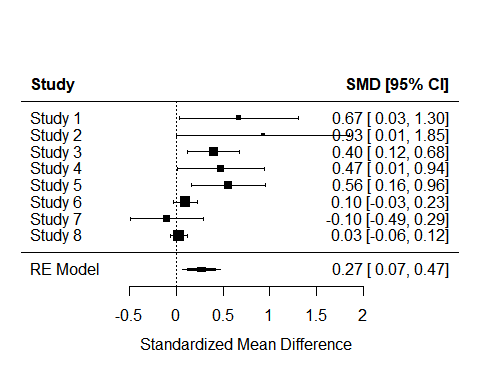
\includegraphics{1_foundational_concepts__lesson_files/figure-latex/unnamed-chunk-14-1.pdf}

\begin{Shaded}
\begin{Highlighting}[]
\FunctionTok{rnorm\_histogram}\NormalTok{(}\AttributeTok{n =} \DecValTok{1000}\NormalTok{, }
                \AttributeTok{mean =} \DecValTok{0}\NormalTok{, }
                \AttributeTok{sd =} \DecValTok{1}\NormalTok{, }
                \AttributeTok{fill =} \StringTok{"darkcyan"}\NormalTok{) }
\end{Highlighting}
\end{Shaded}

\includegraphics{1_foundational_concepts__lesson_files/figure-latex/unnamed-chunk-14-2.pdf}

\begin{Shaded}
\begin{Highlighting}[]
\FunctionTok{rnorm\_histogram}\NormalTok{(}\AttributeTok{n =} \DecValTok{100}\NormalTok{, }
                \AttributeTok{mean =} \DecValTok{0}\NormalTok{, }
                \AttributeTok{sd =} \DecValTok{1}\NormalTok{, }
                \AttributeTok{fill =} \StringTok{"darkorange"}\NormalTok{)}
\end{Highlighting}
\end{Shaded}

\includegraphics{1_foundational_concepts__lesson_files/figure-latex/unnamed-chunk-14-3.pdf}

\hypertarget{test-yourself-is-this-data-normally-distributed}{%
\section{Test yourself: Is this data normally
distributed?}\label{test-yourself-is-this-data-normally-distributed}}

Why or why not?

\begin{Shaded}
\begin{Highlighting}[]
\FunctionTok{set.seed}\NormalTok{(}\DecValTok{238}\NormalTok{)}

\FunctionTok{rnorm\_histogram}\NormalTok{(}\AttributeTok{n =} \DecValTok{50}\NormalTok{, }
                \AttributeTok{mean =} \DecValTok{0}\NormalTok{, }
                \AttributeTok{sd =} \DecValTok{1}\NormalTok{, }
                \AttributeTok{fill =} \StringTok{"darkgreen"}\NormalTok{) }
\end{Highlighting}
\end{Shaded}

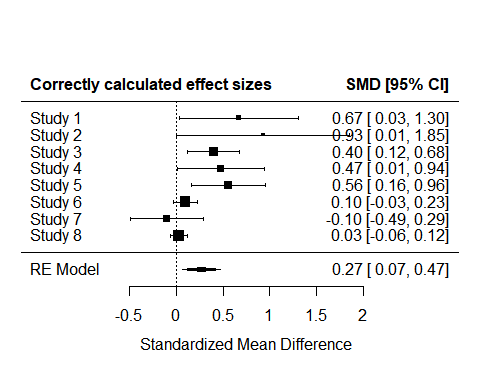
\includegraphics{1_foundational_concepts__lesson_files/figure-latex/unnamed-chunk-15-1.pdf}

\begin{Shaded}
\begin{Highlighting}[]
\FunctionTok{rnorm\_histogram}\NormalTok{(}\AttributeTok{n =} \DecValTok{50}\NormalTok{, }
                \AttributeTok{mean =} \DecValTok{0}\NormalTok{, }
                \AttributeTok{sd =} \DecValTok{1}\NormalTok{, }
                \AttributeTok{fill =} \StringTok{"darkblue"}\NormalTok{) }
\end{Highlighting}
\end{Shaded}

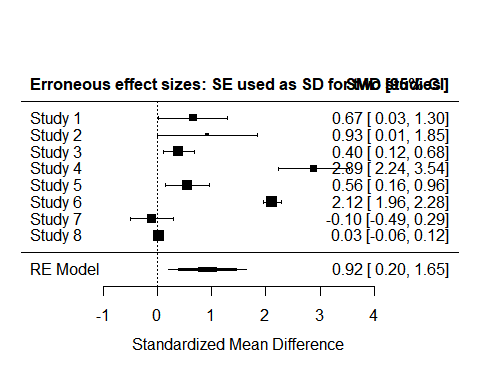
\includegraphics{1_foundational_concepts__lesson_files/figure-latex/unnamed-chunk-15-2.pdf}

\begin{Shaded}
\begin{Highlighting}[]
\FunctionTok{rnorm\_histogram}\NormalTok{(}\AttributeTok{n =} \DecValTok{50}\NormalTok{, }
                \AttributeTok{mean =} \DecValTok{0}\NormalTok{, }
                \AttributeTok{sd =} \DecValTok{1}\NormalTok{, }
                \AttributeTok{fill =} \StringTok{"darkred"}\NormalTok{) }
\end{Highlighting}
\end{Shaded}

\includegraphics{1_foundational_concepts__lesson_files/figure-latex/unnamed-chunk-15-3.pdf}

\hypertarget{simulations-using-for-loops}{%
\section{Simulations using ``for
loops''}\label{simulations-using-for-loops}}

Above, we saw how to simulate data for a single sample, how to plot it
in a histogram, and even how to do both in a single function
(\texttt{simulateR::rnorm\_histogram()}).

Let's do this again using new population parameters: \(\mu\) = 2.25 and
\(\sigma\) = 1. We'll draw 100 samples from this population
distribution. This time, we'll set these population parameters as
variables so they can be reused without having to type them each time.

\begin{Shaded}
\begin{Highlighting}[]
\CommentTok{\# define the parameters}
\NormalTok{n\_samples }\OtherTok{\textless{}{-}} \DecValTok{100} \CommentTok{\# number of samples in each simulation}
\NormalTok{mu }\OtherTok{\textless{}{-}} \FloatTok{2.25}       \CommentTok{\# population mean}
\NormalTok{sigma }\OtherTok{\textless{}{-}} \DecValTok{1}       \CommentTok{\# population standard deviation}

\CommentTok{\# make an annotated histogram}
\FunctionTok{rnorm\_histogram}\NormalTok{(}\AttributeTok{n =}\NormalTok{ n\_samples, }
                \AttributeTok{mean =}\NormalTok{ mu, }
                \AttributeTok{sd =}\NormalTok{ sigma)}
\end{Highlighting}
\end{Shaded}

\includegraphics{1_foundational_concepts__lesson_files/figure-latex/unnamed-chunk-16-1.pdf}

We can also skip the histogram and just simulate the data itself and
then calculate the sample mean and SD. We'll do this using the
parameters set in the previous chunk.

\begin{Shaded}
\begin{Highlighting}[]
\NormalTok{simulated\_scores }\OtherTok{\textless{}{-}} 
    \FunctionTok{rnorm}\NormalTok{(}\AttributeTok{n =}\NormalTok{ n\_samples, }
          \AttributeTok{mean =}\NormalTok{ mu, }
          \AttributeTok{sd =}\NormalTok{ sigma) }

\FunctionTok{mean}\NormalTok{(simulated\_scores) }\SpecialCharTok{|\textgreater{}} \FunctionTok{round\_half\_up}\NormalTok{(}\DecValTok{2}\NormalTok{)}
\end{Highlighting}
\end{Shaded}

\begin{verbatim}
## [1] 2.3
\end{verbatim}

\begin{Shaded}
\begin{Highlighting}[]
\CommentTok{\#sd(simulated\_scores) |\textgreater{} round\_half\_up(2)}
\end{Highlighting}
\end{Shaded}

If you're reading this in the .Rmd file rather than as a .html, click
the run button on the previous chunk a few times to re-run the code.
Notice that the sample mean and SD are different each time. Each one is
somewhat close to the population value, but not exact.

Each time you click run, you are creating a new ``iteration'' of this
very small simulation: the same code, specifying the same population
parameters are generating data, and that data is being analyzed in some
way (in this case: by calculating a mean and SD).

A full-blown simulation study would typically include thousands of
iterations, and conclusions would be made by summarizing across those
thousands of iterations.

\hypertarget{multiple-iterations-of-a-given-simulation}{%
\section{Multiple iterations of a given
simulation}\label{multiple-iterations-of-a-given-simulation}}

What if I wanted to generate these means of simulated data lots of
times?

The following code implements the following logic: ``for the
\texttt{i}th element in the sequence 1 to 10 (i.e., 1, 2, 3, 4, 5, 6, 7,
8, 9, 10), run the following code that appears between the curly
brackets \{\}.

You have seen the code between the curly brackets before above: it
generates normal data from the population parameters, calculates the
sample mean, and prints it. Putting it in a for loop allows us to run it
10 times. This is very useful when you want to run things an arbitrary
and large amount of times, e.g., 10,000.

\begin{Shaded}
\begin{Highlighting}[]
\ControlFlowTok{for}\NormalTok{(i }\ControlFlowTok{in} \DecValTok{1}\SpecialCharTok{:}\DecValTok{10}\NormalTok{)\{}
  \CommentTok{\# generate data sampled from a normal population using rnorm}
\NormalTok{  simulated\_scores }\OtherTok{\textless{}{-}} 
    \FunctionTok{rnorm}\NormalTok{(}\AttributeTok{n =}\NormalTok{ n\_samples, }
          \AttributeTok{mean =}\NormalTok{ mu, }
          \AttributeTok{sd =}\NormalTok{ sigma)}
  
  \CommentTok{\# compute the mean for this simulation and print it}
  \FunctionTok{mean}\NormalTok{(simulated\_scores) }\SpecialCharTok{|\textgreater{}} 
    \FunctionTok{print}\NormalTok{()}
\NormalTok{\}}
\end{Highlighting}
\end{Shaded}

\begin{verbatim}
## [1] 2.345271
## [1] 1.999888
## [1] 2.196017
## [1] 2.329672
## [1] 2.389554
## [1] 2.202022
## [1] 2.250702
## [1] 2.173483
## [1] 2.229205
## [1] 2.217192
\end{verbatim}

Note that the use of \texttt{i} as the iterating variable in a for loop
is just a convention, but it can be any variable. For example, the
following code runs identically:

\begin{Shaded}
\begin{Highlighting}[]
\ControlFlowTok{for}\NormalTok{(whatever\_varible\_name\_you\_want }\ControlFlowTok{in} \DecValTok{1}\SpecialCharTok{:}\DecValTok{10}\NormalTok{)\{ }\CommentTok{\# only this line differs from the previous chunk}
  \CommentTok{\# generate data sampled from a normal population using rnorm}
\NormalTok{  simulated\_scores }\OtherTok{\textless{}{-}} 
    \FunctionTok{rnorm}\NormalTok{(}\AttributeTok{n =}\NormalTok{ n\_samples, }
          \AttributeTok{mean =}\NormalTok{ mu, }
          \AttributeTok{sd =}\NormalTok{ sigma)}
  
  \CommentTok{\# compute the mean for this simulation and print it}
  \FunctionTok{mean}\NormalTok{(simulated\_scores) }\SpecialCharTok{|\textgreater{}} 
    \FunctionTok{print}\NormalTok{()}
\NormalTok{\}}
\end{Highlighting}
\end{Shaded}

\begin{verbatim}
## [1] 2.252013
## [1] 2.270707
## [1] 2.240264
## [1] 2.333123
## [1] 2.317021
## [1] 2.286971
## [1] 2.285349
## [1] 2.292039
## [1] 2.21084
## [1] 2.033861
\end{verbatim}

Note that the loop sequence (previously ``1:10'') can be a variable
instead.

\begin{Shaded}
\begin{Highlighting}[]
\NormalTok{n\_iterations }\OtherTok{\textless{}{-}} \DecValTok{10} 

\ControlFlowTok{for}\NormalTok{(i }\ControlFlowTok{in} \DecValTok{1}\SpecialCharTok{:}\NormalTok{n\_iterations)\{}
  \CommentTok{\# generate data sampled from a normal population using rnorm}
\NormalTok{  simulated\_scores }\OtherTok{\textless{}{-}} 
    \FunctionTok{rnorm}\NormalTok{(}\AttributeTok{n =}\NormalTok{ n\_samples, }
          \AttributeTok{mean =}\NormalTok{ mu,}
          \AttributeTok{sd =}\NormalTok{ sigma)}
  
  \CommentTok{\# compute the mean for this simulation and print it}
  \FunctionTok{mean}\NormalTok{(simulated\_scores) }\SpecialCharTok{|\textgreater{}} 
    \FunctionTok{print}\NormalTok{()}
\NormalTok{\}}
\end{Highlighting}
\end{Shaded}

\begin{verbatim}
## [1] 2.308732
## [1] 2.327487
## [1] 2.108914
## [1] 2.330393
## [1] 2.202904
## [1] 2.257978
## [1] 2.318596
## [1] 2.165976
## [1] 2.203594
## [1] 2.059645
\end{verbatim}

What if I wanted to save the means of simulated data rather than
printing them? Doing anything useful with simulated data will require
that we are able to save results to a usefully formatted data structure.

This takes a bit more effort. Let's take a step back and talk about
assignment, vectors, and for loops.

\hypertarget{assignment-vectors-and-loops}{%
\subsection{Assignment, vectors, and
loops}\label{assignment-vectors-and-loops}}

You already know how variable assignment works. Here we create a new
variable \texttt{n\_iterations} and assign a single integer to it.

\begin{Shaded}
\begin{Highlighting}[]
\NormalTok{n\_iterations }\OtherTok{\textless{}{-}} \DecValTok{10} 

\CommentTok{\# print}
\NormalTok{n\_iterations}
\end{Highlighting}
\end{Shaded}

\begin{verbatim}
## [1] 10
\end{verbatim}

We can also create a vector - a one-dimensional, ordered collection of
values. This numeric vector - ie a vector containing numeric values only
- has \texttt{n\_iterations} number of elements. The elements each take
the default value of 0.

\begin{Shaded}
\begin{Highlighting}[]
\NormalTok{results }\OtherTok{\textless{}{-}} \FunctionTok{numeric}\NormalTok{(n\_iterations)}

\CommentTok{\# print}
\NormalTok{results}
\end{Highlighting}
\end{Shaded}

\begin{verbatim}
##  [1] 0 0 0 0 0 0 0 0 0 0
\end{verbatim}

\begin{Shaded}
\begin{Highlighting}[]
\CommentTok{\# number of elements in the vector == n\_iterations}
\FunctionTok{length}\NormalTok{(results)}
\end{Highlighting}
\end{Shaded}

\begin{verbatim}
## [1] 10
\end{verbatim}

We can alter individual elements of a vector. E.g., we can assign the
first element of this vector to be 5.

\begin{Shaded}
\begin{Highlighting}[]
\NormalTok{results[}\DecValTok{1}\NormalTok{] }\OtherTok{\textless{}{-}} \DecValTok{5}

\CommentTok{\# print}
\NormalTok{results}
\end{Highlighting}
\end{Shaded}

\begin{verbatim}
##  [1] 5 0 0 0 0 0 0 0 0 0
\end{verbatim}

We can also assign the fifth element of this vector to be 4.

\begin{Shaded}
\begin{Highlighting}[]
\NormalTok{results[}\DecValTok{5}\NormalTok{] }\OtherTok{\textless{}{-}} \DecValTok{4}

\CommentTok{\# print}
\NormalTok{results}
\end{Highlighting}
\end{Shaded}

\begin{verbatim}
##  [1] 5 0 0 0 4 0 0 0 0 0
\end{verbatim}

What if we want to assign every element to 7, and we don't want to
repeat ourselves? We can use a for loop.

For the \texttt{i}th element in the sequence 1:n\_iterations (i.e., 1,
2, 3, 4, 5, 6, 7, 8, 9, 10), assign the \texttt{i}th element of the
results vector to be 7.

\begin{Shaded}
\begin{Highlighting}[]
\ControlFlowTok{for}\NormalTok{(i }\ControlFlowTok{in} \DecValTok{1}\SpecialCharTok{:}\NormalTok{n\_iterations)\{}
\NormalTok{  results[i] }\OtherTok{\textless{}{-}} \DecValTok{7}
\NormalTok{\}}

\CommentTok{\# print}
\NormalTok{results}
\end{Highlighting}
\end{Shaded}

\begin{verbatim}
##  [1] 7 7 7 7 7 7 7 7 7 7
\end{verbatim}

What if we want to assign each element not to the same value, but
different values following a pattern? In this case, the value should be
double the value of i.

\begin{Shaded}
\begin{Highlighting}[]
\ControlFlowTok{for}\NormalTok{(i }\ControlFlowTok{in} \DecValTok{1}\SpecialCharTok{:}\NormalTok{n\_iterations)\{}
\NormalTok{  results[i] }\OtherTok{\textless{}{-}}\NormalTok{ i }\SpecialCharTok{*} \DecValTok{2}
\NormalTok{\}}

\CommentTok{\# print}
\NormalTok{results}
\end{Highlighting}
\end{Shaded}

\begin{verbatim}
##  [1]  2  4  6  8 10 12 14 16 18 20
\end{verbatim}

Now let's do something more complex. In the \texttt{i}th iteration of
the loop, we simulate data from a normal distribution, calculate its
mean, and then assign the resulting mean to the \texttt{i}th element of
the results vector.

\begin{Shaded}
\begin{Highlighting}[]
\CommentTok{\# the only difference compared to the first example at the top of the "Multiple iterations of a given simulation" section}
\CommentTok{\# is the resulting means are saved to the results vector.}
\CommentTok{\# But it requires you to think about the loop in a deeper way, and the variable value of i and what its implications are.}
\ControlFlowTok{for}\NormalTok{(i }\ControlFlowTok{in} \DecValTok{1}\SpecialCharTok{:}\NormalTok{n\_iterations)\{}
  \CommentTok{\# generate data sampled from a normal population using rnorm}
\NormalTok{  simulated\_scores }\OtherTok{\textless{}{-}} 
    \FunctionTok{rnorm}\NormalTok{(}\AttributeTok{n =}\NormalTok{ n\_samples, }
          \AttributeTok{mean =}\NormalTok{ mu, }
          \AttributeTok{sd =}\NormalTok{ sigma)}
  
  \CommentTok{\# compute the mean for this simulation and store it }
  \CommentTok{\# in the \textasciigrave{}i\textasciigrave{}th element of the results vector}
\NormalTok{  results[i] }\OtherTok{\textless{}{-}} \FunctionTok{mean}\NormalTok{(simulated\_scores)}
\NormalTok{\}}

\CommentTok{\# print}
\NormalTok{results}
\end{Highlighting}
\end{Shaded}

\begin{verbatim}
##  [1] 2.400711 2.193914 2.298349 2.226627 2.080299 2.137809 2.172315 2.287930
##  [9] 2.283247 2.192627
\end{verbatim}

Now that I have the results of each iteration stored in a vector, I can
also summarize across iterations

\begin{Shaded}
\begin{Highlighting}[]
\CommentTok{\# calculate the mean of means}
\FunctionTok{mean}\NormalTok{(results) }\SpecialCharTok{|\textgreater{}} \FunctionTok{round\_half\_up}\NormalTok{(}\DecValTok{2}\NormalTok{)}
\end{Highlighting}
\end{Shaded}

\begin{verbatim}
## [1] 2.23
\end{verbatim}

\hypertarget{testing-yourself-why-doesnt-this-accomplish-the-goal-of-saving-all-iterations-to-the-vector}{%
\subsection{Testing yourself: Why doesn't this accomplish the goal of
saving all iterations to the
vector?}\label{testing-yourself-why-doesnt-this-accomplish-the-goal-of-saving-all-iterations-to-the-vector}}

To check your own understanding, see if you can guess what output this
code creates and why.

Try to predict what value it returns, and why.

Why doesn't it achieve what the above code does, and what you need it
to? After all, it looks simpler. Indeed, it would be great if it could
accomplish what the previous code does (but it can't).

\hypertarget{parameter-recovery-1}{%
\section{Parameter recovery}\label{parameter-recovery-1}}

Each iteration of a simulation is often intended to correspond with a
semi-realistic real life study or experiment. Real life studies usually
don't have a million participants, maybe they have more like 100. To
know that \texttt{rnorm} is generating data from the population
parameters we tell it to, even in smaller and more realistic sample
sizes where each individual sample isn't very informative, we can check
the long run of studies.

Each individual study will have noise and random variation around it, as
we saw in the histograms above with smaller sample sizes. But the long
run of studies should recover the population parameters. Each iteration
might be relatively small (n\_samples = 100), but we can run a large
number of iterations to average over (n\_iterations = 1000).

\begin{Shaded}
\begin{Highlighting}[]
\CommentTok{\# we increase the number of iterations to simulate a longer run of experiments}
\NormalTok{n\_iterations }\OtherTok{\textless{}{-}} \DecValTok{10000}

\ControlFlowTok{for}\NormalTok{(i }\ControlFlowTok{in} \DecValTok{1}\SpecialCharTok{:}\NormalTok{n\_iterations)\{}
  \CommentTok{\# generate data sampled from a normal population using rnorm}
\NormalTok{  simulated\_scores }\OtherTok{\textless{}{-}} 
    \FunctionTok{rnorm}\NormalTok{(}\AttributeTok{n =}\NormalTok{ n\_samples, }
          \AttributeTok{mean =}\NormalTok{ mu, }
          \AttributeTok{sd =}\NormalTok{ sigma)}
  
  \CommentTok{\# compute the mean for this simulation and store it }
  \CommentTok{\# in the \textasciigrave{}i\textasciigrave{}th element of the results vector}
\NormalTok{  results[i] }\OtherTok{\textless{}{-}} \FunctionTok{mean}\NormalTok{(simulated\_scores)}
\NormalTok{\}}

\CommentTok{\# calculate the mean of means }
\FunctionTok{mean}\NormalTok{(results) }\SpecialCharTok{|\textgreater{}}
  \FunctionTok{round\_half\_up}\NormalTok{(}\DecValTok{2}\NormalTok{)}
\end{Highlighting}
\end{Shaded}

\begin{verbatim}
## [1] 2.25
\end{verbatim}

\begin{Shaded}
\begin{Highlighting}[]
\CommentTok{\# check that the mean of sample means is equal to the population mean (mu)}
\FunctionTok{mean}\NormalTok{(results) }\SpecialCharTok{|\textgreater{}} \FunctionTok{round\_half\_up}\NormalTok{(}\DecValTok{2}\NormalTok{) }\SpecialCharTok{==}\NormalTok{ mu}
\end{Highlighting}
\end{Shaded}

\begin{verbatim}
## [1] TRUE
\end{verbatim}

We can know with greater confidence that our simulations are working by
running an experiment for ourselves: when we change the population
parameters to other values, does the simulation also recover those?
After all, perhaps there is a chance that our simulation (for whatever
reason) simply always returns a mean of means of the same value that we
used as our population parameter.

The code for this simulation is self contained: it doesn't rely on
variables from previous chunks. This is the complete, working
simulation. Not of something very interesting, admittedly: it just
checks that the \(\mu\) and \(\sigma\) values that we pass as arguments
to the \texttt{rnorm()} function do indeed results in datasets with
those means and SDs in the long run. If this were not the case, any
other simulation relying on \texttt{rnorm()} would produce invalid
results.

\begin{Shaded}
\begin{Highlighting}[]
\FunctionTok{set.seed}\NormalTok{(}\DecValTok{42}\NormalTok{)}

\CommentTok{\# new values }
\NormalTok{n\_samples }\OtherTok{\textless{}{-}} \DecValTok{100}
\NormalTok{n\_iterations }\OtherTok{\textless{}{-}} \DecValTok{10000}
\NormalTok{mu }\OtherTok{\textless{}{-}} \SpecialCharTok{{-}}\FloatTok{2.84}
\NormalTok{sigma }\OtherTok{\textless{}{-}} \FloatTok{5.10}

\CommentTok{\# create two new results vectors}
\NormalTok{results\_means }\OtherTok{\textless{}{-}} \FunctionTok{numeric}\NormalTok{(n\_iterations)}
\NormalTok{results\_sds }\OtherTok{\textless{}{-}} \FunctionTok{numeric}\NormalTok{(n\_iterations)}

\ControlFlowTok{for}\NormalTok{(i }\ControlFlowTok{in} \DecValTok{1}\SpecialCharTok{:}\NormalTok{n\_iterations)\{}
  \CommentTok{\# generate data sampled from a normal population using rnorm}
\NormalTok{  simulated\_scores }\OtherTok{\textless{}{-}} 
    \FunctionTok{rnorm}\NormalTok{(}\AttributeTok{n =}\NormalTok{ n\_samples, }
          \AttributeTok{mean =}\NormalTok{ mu, }
          \AttributeTok{sd =}\NormalTok{ sigma)}
  
  \CommentTok{\# compute the mean for this simulation and store it }
  \CommentTok{\# in the \textasciigrave{}i\textasciigrave{}th element of each results vector}
\NormalTok{  results\_means[i] }\OtherTok{\textless{}{-}} \FunctionTok{mean}\NormalTok{(simulated\_scores)}
\NormalTok{  results\_sds[i] }\OtherTok{\textless{}{-}} \FunctionTok{sd}\NormalTok{(simulated\_scores)}
\NormalTok{\}}

\CommentTok{\# compute the mean of means}
\FunctionTok{mean}\NormalTok{(results\_means) }\SpecialCharTok{|\textgreater{}} \FunctionTok{round\_half\_up}\NormalTok{(}\DecValTok{2}\NormalTok{)}
\end{Highlighting}
\end{Shaded}

\begin{verbatim}
## [1] -2.84
\end{verbatim}

\begin{Shaded}
\begin{Highlighting}[]
\CommentTok{\# check that the mean of sample means is equal to the population mean (mu)}
\FunctionTok{mean}\NormalTok{(results\_means) }\SpecialCharTok{|\textgreater{}} \FunctionTok{round\_half\_up}\NormalTok{(}\DecValTok{2}\NormalTok{) }\SpecialCharTok{==}\NormalTok{ mu}
\end{Highlighting}
\end{Shaded}

\begin{verbatim}
## [1] TRUE
\end{verbatim}

\begin{Shaded}
\begin{Highlighting}[]
\CommentTok{\# compute the mean of SDs}
\FunctionTok{mean}\NormalTok{(results\_sds) }\SpecialCharTok{|\textgreater{}} \FunctionTok{round\_half\_up}\NormalTok{(}\DecValTok{2}\NormalTok{)}
\end{Highlighting}
\end{Shaded}

\begin{verbatim}
## [1] 5.09
\end{verbatim}

\begin{Shaded}
\begin{Highlighting}[]
\CommentTok{\# check that the mean of sample SDs is equal to the population SD (sigma)}
\FunctionTok{mean}\NormalTok{(results\_sds) }\SpecialCharTok{|\textgreater{}} \FunctionTok{round\_half\_up}\NormalTok{(}\DecValTok{2}\NormalTok{) }\SpecialCharTok{==}\NormalTok{ sigma}
\end{Highlighting}
\end{Shaded}

\begin{verbatim}
## [1] FALSE
\end{verbatim}

\hypertarget{understanding-this-simulation-in-terms-of-frequentist-statistics-and-vice-versa}{%
\section{Understanding this simulation in terms of frequentist
statistics and
vice-versa}\label{understanding-this-simulation-in-terms-of-frequentist-statistics-and-vice-versa}}

Whether you realized it until now or not, this stimulation follows and
indeed formalizes the same logic as frequentist statistics:

It imagines that smaller, finite studies are run. Each of them have a
realistic number of participants, not the million samples that created
the perfect normal curves in the histograms we saw earlier. Each study
contains both some indication of the data generating signal - the normal
distribution following specific population parameters that gave rise to
the data. At the same time, each study contains much uncertainty and
noise due to its finite size and random chance.

But, in the long run of studies - either a long run of real, actual
replication studies (if unbiased etc), or an arbitrarily long run of
simulation iterations - we can see that the population values are being
uncovered (or recovered, in the case of the simulations).

We have used this simulation to prove that the (incredibly useful)
\texttt{rnorm()} function functions correctly, and generates normally
distributed data following known population means (\(\mu\)) and SDs
(\(\sigma\)).

\hypertarget{simulating-the-false-positive-rate-of-a-t-test}{%
\section{Simulating the false-positive rate of a
t-test}\label{simulating-the-false-positive-rate-of-a-t-test}}

Now that we know \texttt{rnorm()} produces the type of data it claims
to, we can use it for more interesting things.

By definition, a frequentist test's alpha value (e.g., .05) should equal
the test's false-positive rate. But this is not always the case, under
suboptimal conditions. Knowing when and where this is violated tells us
about the assumptions of that test, and therefore the conditions under
which it will work more or less well. Let's simulate 10,000 datasets,
each drawn from a population effect that is null, and check that we do
indeed find significant results in only 5\% of cases (as the alpha value
implies).

Notice that the comments in this code chunk highlight the key components
of a simulation study, similar to that described in Hallgren (2013)
``Conducting Simulation Studies in the R Programming Environment''.

\begin{Shaded}
\begin{Highlighting}[]
\CommentTok{\# set seed for reproducibility}
\FunctionTok{set.seed}\NormalTok{(}\DecValTok{42}\NormalTok{)}

\CommentTok{\# simulation parameters}
\NormalTok{n\_control      }\OtherTok{\textless{}{-}} \DecValTok{50}
\NormalTok{n\_intervention }\OtherTok{\textless{}{-}} \DecValTok{50}
\NormalTok{mu\_control      }\OtherTok{\textless{}{-}} \DecValTok{0} \CommentTok{\# both mu values are zero: population effect is null. }
\NormalTok{mu\_intervention }\OtherTok{\textless{}{-}} \DecValTok{0} 
\NormalTok{sigma\_control      }\OtherTok{\textless{}{-}} \DecValTok{1}
\NormalTok{sigma\_intervention }\OtherTok{\textless{}{-}} \DecValTok{1}
\NormalTok{n\_iterations }\OtherTok{\textless{}{-}} \DecValTok{10000}

\CommentTok{\# create results vector}
\NormalTok{results\_ps }\OtherTok{\textless{}{-}} \FunctionTok{numeric}\NormalTok{(n\_iterations)}

\CommentTok{\# for loop used to repeat this many times}
\ControlFlowTok{for}\NormalTok{(i }\ControlFlowTok{in} \DecValTok{1}\SpecialCharTok{:}\NormalTok{n\_iterations)\{}
  \CommentTok{\# data generation }
\NormalTok{  data\_control      }\OtherTok{\textless{}{-}} \FunctionTok{rnorm}\NormalTok{(}\AttributeTok{n =}\NormalTok{ n\_control,      }\AttributeTok{mean =}\NormalTok{ mu\_control,      }\AttributeTok{sd =}\NormalTok{ sigma\_control)}
\NormalTok{  data\_intervention }\OtherTok{\textless{}{-}} \FunctionTok{rnorm}\NormalTok{(}\AttributeTok{n =}\NormalTok{ n\_intervention, }\AttributeTok{mean =}\NormalTok{ mu\_intervention, }\AttributeTok{sd =}\NormalTok{ sigma\_intervention)}
  
  \CommentTok{\# data analysis}
\NormalTok{  p }\OtherTok{\textless{}{-}} \FunctionTok{t.test}\NormalTok{(}\AttributeTok{x =}\NormalTok{ data\_control, }
              \AttributeTok{y =}\NormalTok{ data\_intervention,}
              \AttributeTok{var.equal =} \ConstantTok{TRUE}\NormalTok{,}
              \AttributeTok{alternative =} \StringTok{"two.sided"}\NormalTok{)}\SpecialCharTok{$}\NormalTok{p.value}
  
\NormalTok{  results\_ps[i] }\OtherTok{\textless{}{-}}\NormalTok{ p}
\NormalTok{\}}

\CommentTok{\# summarise results across iterations}
\CommentTok{\# compute the false positive rate (proportion of significant p values when population effect is null)}
\FunctionTok{mean}\NormalTok{(results\_ps }\SpecialCharTok{\textless{}}\NormalTok{ .}\DecValTok{05}\NormalTok{) }\SpecialCharTok{|\textgreater{}} \FunctionTok{round\_half\_up}\NormalTok{(}\DecValTok{2}\NormalTok{)}
\end{Highlighting}
\end{Shaded}

\begin{verbatim}
## [1] 0.05
\end{verbatim}

Results demonstrate that the false positive rate for a Student's t-test
with 100 participants is indeed 5\%, as implied by the alpha value.
However, there are other situations where this does not hold. If you
like, try changing the simulation parameters and find what combination
of them produce an inflated false-positive rate. We will return to this
question is a later lesson.

\hypertarget{session-info}{%
\section{Session info}\label{session-info}}

\begin{Shaded}
\begin{Highlighting}[]
\FunctionTok{sessionInfo}\NormalTok{()}
\end{Highlighting}
\end{Shaded}

\begin{verbatim}
## R version 4.3.2 (2023-10-31 ucrt)
## Platform: x86_64-w64-mingw32/x64 (64-bit)
## Running under: Windows 11 x64 (build 22631)
## 
## Matrix products: default
## 
## 
## locale:
## [1] LC_COLLATE=German_Switzerland.utf8  LC_CTYPE=German_Switzerland.utf8   
## [3] LC_MONETARY=German_Switzerland.utf8 LC_NUMERIC=C                       
## [5] LC_TIME=German_Switzerland.utf8    
## 
## time zone: Europe/Zurich
## tzcode source: internal
## 
## attached base packages:
## [1] stats     graphics  grDevices utils     datasets  methods   base     
## 
## other attached packages:
##  [1] simulateR_0.1    janitor_2.2.0    kableExtra_1.4.0 knitr_1.46      
##  [5] scales_1.3.0     lubridate_1.9.3  forcats_1.0.0    stringr_1.5.1   
##  [9] dplyr_1.1.4      purrr_1.0.2      readr_2.1.5      tidyr_1.3.1     
## [13] tibble_3.2.1     ggplot2_3.5.1    tidyverse_2.0.0 
## 
## loaded via a namespace (and not attached):
##  [1] gtable_0.3.5        xfun_0.43           lattice_0.21-9     
##  [4] numDeriv_2016.8-1.1 mathjaxr_1.6-0      tzdb_0.4.0         
##  [7] quadprog_1.5-8      vctrs_0.6.5         tools_4.3.2        
## [10] generics_0.1.3      stats4_4.3.2        parallel_4.3.2     
## [13] fansi_1.0.6         highr_0.10          pkgconfig_2.0.3    
## [16] Matrix_1.6-1.1      lifecycle_1.0.4     farver_2.1.1       
## [19] compiler_4.3.2      munsell_0.5.1       mnormt_2.1.1       
## [22] codetools_0.2-19    snakecase_0.11.1    htmltools_0.5.8.1  
## [25] yaml_2.3.8          pillar_1.9.0        furrr_0.3.1        
## [28] metadat_1.2-0       nlme_3.1-163        parallelly_1.37.1  
## [31] lavaan_0.6-17       tidyselect_1.2.1    digest_0.6.35      
## [34] stringi_1.8.3       future_1.33.2       listenv_0.9.1      
## [37] labeling_0.4.3      fastmap_1.1.1       grid_4.3.2         
## [40] colorspace_2.1-0    cli_3.6.2           metafor_4.6-0      
## [43] magrittr_2.0.3      utf8_1.2.4          broom_1.0.5        
## [46] future.apply_1.11.2 pbivnorm_0.6.0      effsize_0.8.1      
## [49] withr_3.0.0         backports_1.4.1     timechange_0.3.0   
## [52] rmarkdown_2.26      globals_0.16.3      hms_1.1.3          
## [55] evaluate_0.23       viridisLite_0.4.2   rlang_1.1.3        
## [58] glue_1.7.0          xml2_1.3.6          svglite_2.1.3      
## [61] rstudioapi_0.16.0   R6_2.5.1            systemfonts_1.0.6
\end{verbatim}

\end{document}
